
% Works
% -----

\subsection{Conditional Operation and Inverse Sequences}

\begin{mydef}[Sets of sequences]
As we will frequently refer to sets of fequences,
we will use calligraphic letters (e.g. $\seqset{A, B, C}$ and $\seqset{S}$)
to denote such sets for brevity.
We will use $A\cc\seqset{B}$ to denote the set of sequences $\{A\cc B|B\in\seqset{B}\}$.
\end{mydef}

\begin{mydef}[$\Dom{X}$ and $\Img{X}$]
$\Dom{X}$ is the domain of $X$.
For a sequence of commands $A$, $\Dom{A}$ is the set of filesystems $A$ does not break.
For a set of sequences $\seqset{A}$, $\Dom{\seqset{A}}$ is the set of filesystems no $A\in\seqset{A}$ breaks.
We write $\Img{X}$ to denote the image of the domain of the sequence $X$.
\end{mydef}

\begin{mydef}[$\worksmsign$, $\worksmeqsign$]
For two sets of sequences $\sqs{A}$ and $\sqs{B}$
we write $\worksm{\sqs{A}}{\sqs{B}}$ iff $\Dom{\sqs{A}} \subseteq \Dom{\sqs{B}}$;
that is, if all sequences in $\sqs{B}$ work (do not break the filesystem)
on any filesystem all sequences in $\sqs{A}$ work on.
We write $\worksmstr{\sqs{A}}{\sqs{B}}$ iff $\Dom{\sqs{A}} \subset \Dom{\sqs{B}}$.

As a special case, we write $\worksmnil{\sqs{A}}$ if we know that there is a filesystem
all sequences in $\sqs{A}$ work on,
and we apply these relations to sequences directly:
$\worksm{A}{B}$ with the meaning $\worksm{\{A\}}{\{B\}}$.
\end{mydef}

It is easy to see that the following corollaries are true:

\begin{mycor}\label{worksextpostfix}
% An inference rule in the algebra
$\forall A,S: \worksm{A\cc S}{A}$, that is, if a sequence works, its initial segment also works.
\end{mycor}

\begin{mycor}\label{workschained}
% An inference rule in the algebra
$\worksmeqsign$ can be chained:
if $\seqset{B'}\subseteq\seqset{B}$, then
$\worksm{\sqs{A}}{\sqs{B}} \wedge \worksm{\sqs{B'}}{\sqs{C}} \Rightarrow \worksm{\sqs{A}}{\sqs{B}\cup\sqs{C}}$.
\end{mycor}

We also prove the following lemmas.

\begin{myax}\label{combine_independent_commands}
The combination of independent commands works wherever the original commands work:
\[ \alpha\indep \beta \Rightarrow \worksm{\{\alpha, \beta\}}{\{\alpha\cc \beta\}}. \]
\end{myax}
\begin{proof}
We name this proposition a \namecref{combine_independent_commands} 
because to prove it, we must reach back to our filesystem model.
Let $\alpha=\cxynv$ and $\beta=\czwmv$.
%% TODO by contradiction
We proceed in an indirect way and
assume that there is a filesystem $\FS$ for which
$\cxynv\aFS\neq\fsbroken$ and $\czwmv\aFS\neq\fsbroken$, but
$\cxynv\cc \czwmv\aFS=\fsbroken$.
We know $\cxynv\aFS\neq\fsbroken$ so it must be applying 
$\czwmv$ that breaks it.
Applying a command can only result in a broken filesystem in three cases.
First, if the filesystem was already broken, which cannot be the case here.
Second, if the input type does not match the filesystem,
but we know $[\FS(m)]=[w]$ and so
$[(\cxynv\aFS)(m)]=[w]$ as based on \cref{incomparable_is_independent}, $n\neq m$.
Third, if the new filesystem violates the tree property.
This again cannot be the case because we also know that $n\unrel m$
and the tree property only depends on the types of the parent and children of $m$,
which therefore cannot be changed by $\cxynv$.
\end{proof}

This result can be extended to sequences:

\begin{mylem}\label{combine_independent_sequences}
The combination of independent sequences works wherever the original sequences work:
\[ S\indep T \Rightarrow \worksm{\{S,T\}}{\{S\cc T\}}. \]
\end{mylem}
\begin{proof}
Assume that there is a filesystem $\FS$ so that
$S\aFS\neq\fsbroken$ and $T\aFS\neq\fsbroken$, but
$(S\cc T)\FS=\fsbroken$.

From \cref{incomparable_is_independent,ax_separate_commute} we know that
the commands in $S$ and $T$ pairwise commute, and so any sequence
that contains the commands from $S$ and $T$ and preserve their original partial order
is equivalent to $S\cc T$ on all filesystems.

Let the command that breaks $\FS$ in $T$ when applying $S\cc T$ be $t$
so that $T=T_0\cc t\cc T_1$.
It is still true that $(T_0 \cc t)\FS\neq\fsbroken$,
and by definition $(S\cc T_0)\FS\neq\fsbroken$,
but $(S\cc T_0\cc t)\FS=\fsbroken$.
Also, from above we know that $S\cc T_0\equiv T_0\cc S$
and so $(T_0 \cc S)\FS\neq\fsbroken$.

If we denote the first command in $S$ with $s_1$,
this means that $(T_0 \cc s_1)\FS\neq\fsbroken$,
which we can combine with $(T_0 \cc t)\FS\neq\fsbroken$, $t\indep s_1$ and
\cref{combine_independent_commands}
(using $T_0\FS$ as the reference filesystem)
to arrive at $(T_0 \cc s_1\cc t)\FS\neq\fsbroken$.

We can repeat this step for $s_2$, the next command in $S$,
and from 
$(T_0 \cc s_1\cc t)\FS\neq\fsbroken$
and
$(T_0 \cc s_1\cc s_2)\FS\neq\fsbroken$
arrive at
$(T_0 \cc s_1\cc s_2\cc t)\FS\neq\fsbroken$.
This can be repeated until $S$ is exhausted and we get
$(T_0 \cc S\cc t)\FS\neq\fsbroken$, which is a contradiction.
\end{proof}

We also prove the following:

\begin{mylem}\label{worksinputmatch}
If $A$ and $B$ are minimal sequences, $\worksmnil{\{A,B\}}$,
and there are commands on node $n$ in both $A$ ($\cxynv\in A$) and $B$ ($\czwnv\in B$),
then the input types of these commands must match ($[x]=[z]$).
\end{mylem}
\begin{proof}
This result is similar to \cref{equiv_simple_same_commands} and
%% TODO by contradiction
is easily shown using an indirect proof: if $[x]\neq [z]$, then there is no filesystem that
either $\cxynv$ or $\czwnv$ would not break, 
and consequently $A$ and $B$ cannot work on the same filesystem.
\end{proof}


\bigskip

%% TODO https://en.wikipedia.org/wiki/Equivalence_class

\noindent
We know that whether commands break a filesystem depends solely on their input and output
types and the node, but not their actual output value.
To represent this, we introduce an equivalence relation between filesystems, commands
and sequences of commands.
%% TODO extending it!
\begin{mydef}[Equivalence by type: $\typeeq$]
$ $ % otherwise first list element starts on same line
\begin{itemize}
\item For two filesystems $\FS\typeeq\GS$ iff they are both broken, or they share the same nodes $\setn$,
and for all $n\in\setn$, $\FS(n) \typeeq \GS(n)$.
\item For two commands $\cxynv\typeeq\czwnv$ iff 
$x\typeeq z$ and $y\typeeq w$ and $n=m$.
\item For two sequences of commands $\emptyseq\typeeq\emptyseq$, and
if $A'=\alpha\cc A$ and $B'=\beta\cc B$, then $A'\typeeq B'$ iff $\alpha\typeeq\beta$ and $A\typeeq B$.
\end{itemize}
\end{mydef}

We select representatives of each $\typeeq$-equivalence class of values:
for $[\empt]$ and $[\vald]$ this must be $\empt$ and $\vald$; and
for $[\valf]$ we select an arbitrary file value $\fil\in[\valf]$.
We then use these representative values to
introduce the canonical mapping $\T$ that preserves the types of values,
but maps all objects into a subsystem where there is a one-to-one
correspondence between types and values.

\begin{mydef}[$\T$]
We use $\T$ and write $X\T$ to denote the canonical mapping of 
values, filesystems, commands and sequences to the
representatives of their $\typeeq$-equivalence class.
\begin{itemize}
\item For values, $\vald\T=\vald$, $\valf\T=\fil$ and $\empt\T=\empt$.
\item For filesystems, $\fsbroken\T=\fsbroken$ and in other cases $\FS\T$ is defined by $\FS\T(n) = \FS(n)\T$.
\item For commands, $\cbrk\T=\cbrk$ and $\cxynv\T = \cTxynv$.
\item For sequences of commands, $\emptyseq\T=\emptyseq$, and if $S'=\alpha\cc S$, then $S'\T=\alpha\T\cc S\T$.
\item Finally we extend $\T$ to sets of sequences: $\seqset{A}\T = \{S\T | S\in\seqset{A}\}$.
\end{itemize}
\end{mydef}

It is easy to see that for all objects where it is defined, $X\T\typeeq X$.
% $|\setf|$ is also $1$.
As representatives of filesystems, commands, sequences, etc.
are subsets of their non-representative counterparts, all
propositions proven so far apply to them as well.

\begin{mycor}
For any filesystem $\FS$ and command $\alpha$, 
$\alpha\T(\FS\T) = (\alpha\aFS)\T$.
TODO needed?
\end{mycor}

% It is easy to see that 
% $A\equiv B \Rightarrow A\T\equiv B\T$ 
% and
% $A\eqext B \Rightarrow A\T\eqext B\T$,
% but the reverse is not true as 
% $A\T$ and $B\T$ will have the same effect on all filesystems
% if $A$ and $B$ differ only in some of the values in their commands,
% whereas clearly $A\nequiv B$.

As whether a sequence of commands breaks a filesystem does not depend on the output values
of the commands, only the input and output types, we know that
\begin{mycor}\label{repr_works_is_same}
\begin{gather*}
\works{\seqset{A}} \Leftrightarrow \works{\seqset{A}\T} \\
\worksc{\seqset{A}}{\seqset{B}} \Leftrightarrow \worksc{\seqset{A}\T}{\seqset{B}\T}.
\end{gather*}
\end{mycor}


We are now ready to define the inverse of representative commands $\alpha\T$
which allows us to move parts of sequences between the
condition and consequence parts of $\workssign$.
This is based on the following observation.

\begin{mylem}\label{repr_comm_inject}
Representative commands $\alpha\T$ are injections over representative filesystems ($\FS\T$)
except for the cases where they break a filesystem, that is,
\[ \forall\FS,\GS,\alpha: \FS\T\neq\GS\T \wedge \alpha\T(\FS\T)\neq\fsbroken \Longrightarrow \alpha\T(\FS\T) \neq \alpha\T(\GS\T). \]
\end{mylem}
\begin{proof}
This is trivial if $\GS\T=\fsbroken$, so we assume it is not so.
Let $\alpha\T = \cTxynv$.
If $\FS\T$ and $\GS\T$ have different values at any node apart from $n$, then this difference remains
even after applying $\cTxynv$ to $\FS\T$. The only remaining case therefore is where they have the same values
at all nodes except $n$.
As $\cTxynv(\FS\T)\neq\fsbroken$, we know $[\FS\T(n)]=[x]$.
We also know that $\GS\T(n)\neq\FS\T(n)$, and therefore, as there is a one-to-one correspondence between values and types,
$[\GS\T(n)]\neq[x]$.
This implies $\cTxynv(\GS\T)=\fsbroken$,
and again we have $\alpha\T(\FS\T) \neq \alpha\T(\GS\T)$.
\end{proof}

% TODO We introduced BREAK to deal with cases where commands
% are in effect not defined. Now we need to undo this 
% to see that repr commands are bijective.

\begin{mydef}[Inverse commands and sequences]
If based on \cref{repr_comm_inject}
we regard the representative command $\alpha\T$ a bijective function whose
domain is the subset of representative filesystems $\{\FS\T | \alpha\aFS\neq\fsbroken\}$,
then we can define the inverse of $\alpha\T$
for which we write $\alpha\T^{-1}$.
For any $\GS\T$ outside the image of the domain of $\alpha\T$ we define $\alpha\T^{-1}(\GS\T)$ to be $\fsbroken$.

We write ${S\T}^{-1}$ for the inverse of the sequence $S\T$, which consists of the inverses of the commands in $S\T$
in reverse order.
\end{mydef}

%% TODO
% Do we need <[x],[y],n>-1 = <[y],[x],n> ?
% Do we need to prove if a filesystem is not in the image, then a-1 will break it?
\begin{mylem}
For representative commands
\[ \cTxynv^{-1} = \cTyxnv. \]
\end{mylem}
TODO needed? -maybe for \cref{negneg_is_typeeq}

From the definitions we can clearly see that
\begin{mycor}\label{negneg_is_typeeq}
$\forall S: ({S\T}^{-1})^{-1} = S\T$.
\end{mycor}

For brevity, in the following lemma we use $B$, $B'$, $\seqset{A}$ and $\seqset{C}$ to denote
representative sequences and sets.

\begin{mylem}\label{r_invmove}
A common initial segment of a set of \emph{representative} sequences can be moved to the other side of $\worksmeqsign$ by inverting it:
\begin{gather*}
\worksm{\seqset{C}}{B\cc \seqset{A}}
\ \Longleftrightarrow \ \worksm{B^{-1}\cc \seqset{C}}{\seqset{A}} 
\ \wedge \  \worksm{\seqset{C}}{\{B\}}
\end{gather*}
\end{mylem}
\begin{proof}
% TODO Rewrite for equivalence, and swap A and C.
% This result is quite expected as we're mapping a subset statement using a bijection,
% but made more complicated a as B is not defined everywhere.

The proof for both propositions is illustrated by \cref{fig_invmove}.

\begin{figure}[htb]
\begin{center}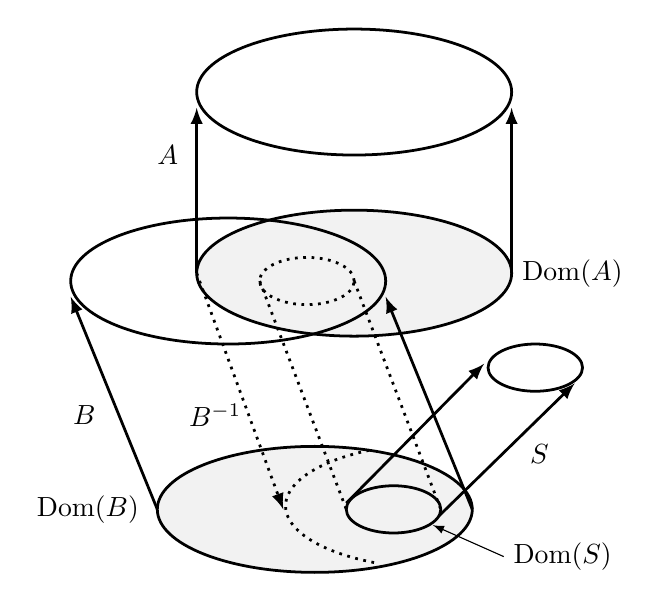
\begin{tikzpicture}
[line width=1pt]
\node at  (1.6+2, 0.1) [right] {$\textrm{Dom}(\seqset{A})$};
\draw[fill=black!5] (1.6, 0.1) ellipse (2cm and 0.8cm); %% Dom A
\draw               (1.6, 2.4) ellipse (2cm and 0.8cm); %% Img A
\draw[-latex] (1.6+2, 0.1)--(1.6+2, 2.4-.2); %% A right
\draw[-latex] (1.6-2, 0.1)--(1.6-2, 2.4-.2); %% A left
\node at  (1.6-2-.1, 1.6) [left] {$A$};
%%
\node at (1.1-2-.1, -2.9) [left] {$\textrm{Dom}(B)$};
\draw[fill=black!5] (1.1, -2.9) ellipse (2cm and 0.8cm); %% Dom B
\draw               (0  ,  0)   ellipse (2cm and 0.8cm); %% Img B
\draw[-latex] (1.1+2, -2.9)--(0+2, 0-.2); %% B right
\draw[-latex] (1.1-2, -2.9)--(0-2, 0-.2); %% B left
\node at  (0.55-2-.1, -1.7) [left] {$B$};
\draw[-latex,dotted] (1.6-2, 0.1)--(0.7, -2.9); %% B-1
\node at (0.3, -1.7) [left] {$B^{-1}$};
\draw[dotted] (1.79, -2.15) arc(118:244: 2cm and 0.8cm); %% Arc
\draw[dotted] (1, 0) ellipse (0.6cm and 0.3cm); %% Dotted S
\draw         (2.1, -2.9) ellipse (0.6cm and 0.3cm); %% Dom S
\draw[dotted] (1-0.6, 0)--(2.1-0.6, -2.9); %% B-1
\draw[dotted] (1+0.6, 0)--(2.1+0.6, -2.9); %% B-1
\draw                     (3.9, -1.1) ellipse (0.6cm and 0.3cm); %% Img S
\draw[-latex] (2.1-0.6, -2.9+.08)    --(3.9-0.6-.05, -1.1+.05); %% Left S
\draw[-latex] (2.1+0.6-.02, -2.9-.08)--(3.9+0.6-.1, -1.1-.2); %% Right S
\node at  (3.7,-2.2) [right] {$S$};
\draw[-latex,thin] (3.5, -3.5) node[right]{$\mathrm{Dom}(\seqset{S})$} -- (2.1+0.5, -2.9-0.2);
\end{tikzpicture}\end{center}

\caption{Proof of \cref{r_invmove}}\label{fig_invmove}
\end{figure}

Unless $\works{\seqset{C}}$, both propositions are trivially true. Otherwise,
for the first proposition
we know $\works{B\cc\seqset{A}}$, which implies that $\Dom{\seqset{A}}$ intersects with $\Img{B}$ 
as otherwise $B\cc\seqset{A}$ would break all filesystems.
As the (representative) $B$ is a bijection between its domain and image,
we can use $B^{-1}$ to map this intersection back
onto the domain of $B$ and get $\Dom{B\cc\seqset{A}}$.
As $\worksc{B\cc \seqset{A}}{\seqset{C}}$, 
we know that $\Dom{\seqset{C}} \subseteq \Dom{B\cc\seqset{A}}$.
We now use $B$ to map both sides of this statement, which yields
$\Dom{B^{-1}\cc \seqset{C}} \subseteq \Dom{B^{-1}\cc B\cc\seqset{A}}$,
but the latter is a subseteq of $\Dom{\seqset{A}}$,
and so $\Dom{B^{-1}\cc \seqset{C}} \subseteq \Dom{\seqset{A}}$,
from which $\worksc{\seqset{A}}{B^{-1}\cc \seqset{C}}$.

For the second proposition, 
from $\worksc{B}{\seqset{C}}$ we know $\Dom{\seqset{C}} \subseteq \Dom{B}$.
Therefore we can project the whole of $\Dom{\seqset{C}}$ using the bijective representative sequence $B$
to get $\Dom{B^{-1}\cc\seqset{C}}$, and as $\worksc{\seqset{A}}{B^{-1}\cc \seqset{C}}$
we know
$\Dom{B^{-1}\cc\seqset{C}} \subseteq \Dom{\seqset{A}}$.
We use $B^{-1}$ to project both sides of this statement to get
$\Dom{B\cc B^{-1}\cc\seqset{C}} \subseteq \Dom{B\cc\seqset{A}}$.
But we also know that $\Dom{B\cc B^{-1}\cc\seqset{C}} = \Dom{\seqset{C}}$
as $\Dom{\seqset{C}} \subseteq \Dom{B}$,
and so $\Dom{\seqset{C}} \subseteq \Dom{B\cc\seqset{A}}$
from which $\worksc{B\cc \seqset{A}}{\seqset{C}}$.
\end{proof}


\begin{mylem}\label{indep_prefix_combine}
The combination of sequences with a common head and independent tails 
continues to work under the same conditions:
\[ \worksc{A\cc B}{\seqset{S}} \wedge \worksc{A\cc C}{\seqset{S}} \wedge B\indep C \Rightarrow \worksc{A\cc B\cc C}{\seqset{S}} \]
\end{mylem}
\begin{proof}
Based on \cref{repr_works_is_same} we have
$\worksc{A\T\cc B\T}{\seqset{S\T}}$ and $\worksc{A\T\cc C\T}{\seqset{S\T}}$,
and from \cref{r_invmove} we know
$\worksc{B\T}{{A\T}^{-1}\cc \seqset{S\T}}$ and $\worksc{C\T}{{A\T}^{-1}\cc \seqset{S\T}}$.
Using \cref{combine_independent_sequences} we get
$\worksc{B\T\cc C\T}{B\T,C\T}$,
and combining these using \cref{workschained}
we get
$\worksc{B\T\cc C\T}{{A\T}^{-1}\cc \seqset{S\T}}$.

From $\worksc{A\cc B}{\seqset{S}}$ we also know $\worksc{A}{\seqset{S}}$ and $\worksc{A\T}{\seqset{S\T}}$.
We can combine this and $\worksc{B\T\cc C\T}{{A\T}^{-1}\cc \seqset{S\T}}$ using
the second proposition of \cref{r_invmove} to get
$\worksc{A\T\cc B\T\cc C\T}{\seqset{S\T}}$, and from \cref{repr_works_is_same} we know
$\worksc{A\cc B\cc C}{\seqset{S}}$.
\end{proof}
